% Ubah judul dan label berikut sesuai dengan yang diinginkan.
\section{TESTING AND ANALYSIS}
\label{sec:pengujiananalisa}

In this study, the results of the tests and analyzes carried out are presented in accordance with the system design that has been designed in the previous chapter. For testing and analysis, the \textit{Dataset} used is the dataset from \url{https://github.com/meisaputri21/Indonesian-Twitter-Emotion-Dataset}. The test is carried out in several parts as follows:

\begin{enumerate}[nolistsep]
    \item Performance Testing based on Extracted Words
    \item Performance Testing based on the BERT model used
    \item Performance Testing based on the BERT model used
    \item Performance Testing based on the \textit{Training} Approach.
\end{enumerate}

\subsection{Model Performance Test Configuration}

The current capacity of \textit{BERT} can only process 512 words of Tokens, however, because the \textit{Dataset} used has less text characteristics than normal text datasets, 280 words of Tokens are taken. These 280 words are taken because they match the maximum character \textit{Twitter} if the user wants to send a \textit{tweet}.

Performance testing on words that have been taken. The tokens that have been taken aim to determine the accuracy of the \textit{BERT} model in the text. Because tokenized sentences have shorter words, there is no need to cut the word fragments because they are still in the capacity of \textit{BERT} to process tokens, which is 512 words. From the tokenized \textit{Dataset}, several \textit{Parameters} were selected which were considered the most accurate among the other \textit{Parameters} to be entered into the \textit{BERT} model, including \textit{epoch, batch , learning rate, hidden dropout, and epsilon}.

For some \textit{Pretrained Model}, they generally use the same parameters, but there are conditions where different parameters must be used because the \textit{Pretrained Model} directive specification requires that one of the models must use a parameter with a certain value, for example \textit {epsilon} which requires using the values 1e-8.

The output of the model will be compared with the labels in the dataset, which will then be calculated to produce \textit{confusion matrix}, \textit{recall, precision, accuracy} and \textit{f1-score} according to the formula described in the literature review chapter. summarized by a tool, namely \textit{Classification Report}.

\subsection{Model Performance Test Sharing Scheme}

In the \textit{Training} process, it is divided into 4 parts. The first is a test scheme using \textit{Dataset} which does not go through the \textit{Stemming} process or is called \textit{non-stemming} and does not use \textit{Freeze Parameter}, the second is a test scheme using \textit{ The dataset} which does not go through the \textit{Stemming} process or is called \textit{non-stemming} but uses \textit{Freeze Parameter}, the third is \textit{Dataset} which goes through the \textit{Stemming} process and does not use \textit {Freeze Parameter}, and the last one is \textit{Dataset} which goes through the \textit{Stemming} process and uses \textit{Freeze Parameter}.

This scheme was chosen because during testing we wanted to know how accurate a model \textit{BERT} would be if \textit{Dataset} had different treatments as already mentioned. The \textit{Stemming} process as described in the previous chapter is the process of converting affixed words into basic words. Examples such as holding back is holding, and reciprocating to be reciprocated. Here the test is carried out to find out whether the model will produce different accuracy because there are some parts of the affix that are omitted. \textit{Stemming} is done considering that the \textit{Dataset} used is a sentence taken from an Indonesian user \textit{Twitter} where there are many sentences or words that are not standard.

Next is \textit{Freeze Parameters}. \textit{Freeze Parameter} is a condition where the layer or \textit{Layer} is "frozen" or disabled for the purpose of \textit{Training} so that the model created becomes simpler. The \textit{Freeze Parameter} process is carried out whether there is a performance difference between the \textit{BERT} model which has a more complex model and a simpler model. For the \textit{Pretrained Model} used in the \textit{Training} process this time there are 3 pieces sourced from \textit{website} \url{https://huggingface.co/}, where these models are the models used devoted to training the Indonesian language \textit{Twitter} text classification based on the resulting \textit{Emotion}. The following are the models used in the \ref{tab:list_model} table below: 

\begin{table}[!h]
    \caption{\textit{Pretrained Model} used in the test process}
    \label{tab: daftar_model}
    \centering
    \begin{tabular}{|l||l|}
        \hline
       \textbf{Model COde} &\textbf{List of \textit{Pretrained Model}} \\ \hline
        Model 1            &akahana/indonesia-emotion-roberta\\ \hline 
        Model 2            &indolem/indobertweet-base-uncased  \\ \hline
        Model 3            &StevenLimcorn/indonesian-roberta-base-emotion-classifier  \\ \hline 
    \end{tabular}
\end{table}

\subsection{Testing Dataset \textit{Non-Stemming} and Without \textit{Freeze Parameter}}

Testing with the first schema is done with \textit{Dataset} which does not go through the \textit{Stemming} process and without using \textit{Freeze Parameter}. This test does not go through any \textit{Preprocessing} which automatically makes it go straight through the \textit{Training} process. From the three models used, the model performance is as follows:

\begin{figure}[h]
    \begin{center}
        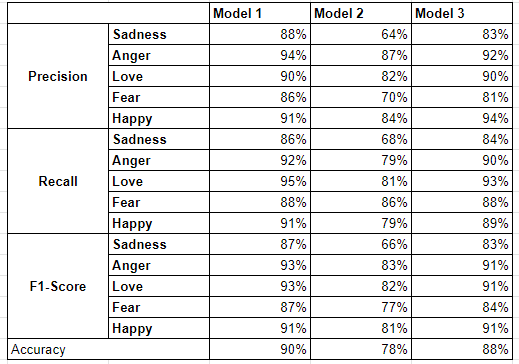
\includegraphics[width= 0.9\linewidth]{template-paper-ieee-main/gambar/1.non_stemming_non_freeze.png}
        \caption{Experimental results of the \textit{Non-Stemming} method and without the \textit{Freeze Parameter} using 3 \textit{Pretrained Model}}
        \label{fig: bertToken}
    \end{center}
\end{figure}

From the experiments carried out, there were several results in the form of the \textit{Metrics} value of the three \textit{Pretrained Model} used. Experiments using the \textit{akahana/indonesia-emotion-roberta} model showed very good results with an accuracy of 90\% and the values \textit{Precision}, \textit{Recall}, and \textit{F1-score} were not there is less than 80\% where this result is classified as very good, but in calculating the difference in \textit{Loss} between \textit{Evaluation} and \textit{Training}, the distance is quite far from \textit{Training loss} always decreases with with increasing \textit{epoch}, but \textit{Evaluation Loss} tends to increase as \textit{epoch} increases.

Experiments using the \textit{indolem/indobertweet-base-uncased} model showed results with an accuracy of 78\% where each value between \textit{Precision}, \textit{Recall}, and \textit{F1-Score} showed values that are varied but are in the range of 64\% the lowest and 87\% the highest. The difference in \textit{Loss} in this model is that \textit{Training Loss} always decreases with increasing \textit{epoch} but for \textit{Evaluation Loss} the value from one \textit{epoch} to another \textit{epoch} tends to stagnate .

Experiments using the \textit{StevenLimcorn/indonesian-roberta-base-emotion-classifier} model more or less produce values that are not much different from those used with the \textit{akahana/indonesia-emotion-roberta} model where the accuracy is 88\%. The value between \textit{Precision}, \textit{Recall}, and \textit{F1-Score} also shows good results where the lowest value is at 81\%, namely the \textit{Precision} value of the \textit{ label Fear} and the highest value is in \textit{Precision} of the label \textit{Happy} with a value of 94\%. Meanwhile, the difference in loss is not much different from the results produced by the \textit{indolem/indobertweet-base-uncased} model where the difference in \textit{Loss} in this model is that \textit{Training Loss} always decreases with increasing \textit{epoch } but for \textit{Evaluation Loss} the value from one \textit{epoch} to another \textit{epoch} tends to stagnate.

\subsection{Testing Dataset \textit{Non-Stemming} and using \textit{Freeze Parameter}}

Testing with the second scheme is carried out with \textit{Dataset} which does not go through the \textit{Stemming} process and uses \textit{Freeze Parameter}. In this Test some \textit{Layer} of the \textit{BERT} Model is disabled in order to produce a simpler model. From the three models used, the model performance is as follows:

\begin{figure}[h]
    \begin{center}
        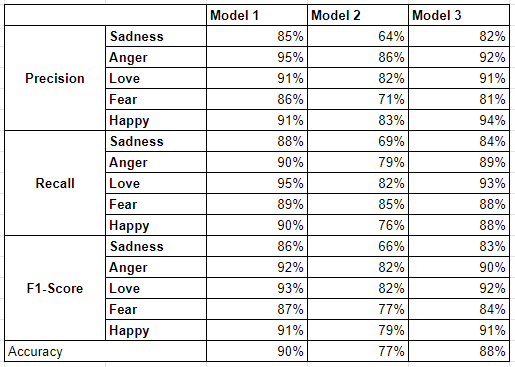
\includegraphics[width= 0.9\linewidth]{template-paper-ieee-main/gambar/2.non_stemming_freeze.png}
        \caption{Experiment results using \textit{Non-Stemming} method and using \textit{Freeze Parameter} using 3 \textit{Pretrained Model}}
        \label{fig: bertToken}
    \end{center}
\end{figure}

Experiments using the \textit{Non-Stemming} Dataset and using the \textit{Freeze Parameter} obtained some results from the three \textit{Pretrained Model} used. First, by using the \textit{akahana/indonesia-emotion-roberta} model, the accuracy results are 90\% where the values \textit{Precision}, \textit{Recall}, and \textit{F1-Score} are not much different from the results obtained. obtained with Dataset \textit{Non-Stemming} which does not use \textit{Freeze Parameter} with a range of 85\% to 95\%. for the amount of difference \textit{loss} between \textit{Evaluation} and \textit{Training}, the distance is quite large with \textit{Training loss} always decreasing as \textit{Epoch} increases, but \textit{Evaluation Loss} tends to increases as \textit{epoch} increases.

Experiments using \textit{indolem/indobertweet-base-uncased} showed more or less the same as the previous experiment, using the \textit{Non-Stemming} Dataset and without using \textit{Freeze Parameter} with an accuracy of 78\%. The values between \textit{Precision}, \textit{Recall}, and \textit{F1-Score} show results in the range of 64\% to 85\% and the \textit{Loss} difference in this model is \textit{Training Loss} always decreases with increasing \textit{epoch} but for \textit{Evaluation Loss} the value from one \textit{epoch} to another \textit{epoch} tends to stagnate.

Experiments using the \textit{StevenLimcorn/indonesian-roberta-base-emotion-classifier} model more or less produce values that are not much different from those used with the \textit{akahana/indonesia-emotion-roberta} model where the accuracy is 88\%. The value between \textit{Precision}, \textit{Recall}, and \textit{F1-Score} also shows good results where the lowest value is at 81\%, namely the \textit{Precision} value of the \textit{ label Fear} and the highest value is in \textit{Precision} of the label \textit{Happy} with a value of 94\%. Meanwhile, the difference in loss is not much different from the results produced by the \textit{indolem/indobertweet-base-uncased} model where the difference in \textit{Loss} in this model is that \textit{Training Loss} always decreases with increasing \textit{epoch } but for \textit{Evaluation Loss} the value from one \textit{epoch} to another \textit{epoch} tends to stagnate.

\subsection{Testing Dataset \textit{Stemming} and without using \textit{Freeze Parameter}}

Testing with the third scheme is carried out with \textit{Dataset} which goes through the \textit{Stemming} process and without using \textit{Freeze Parameter}. In this test \textit{Dataset} goes through the \textit{Stemming} process and as a result the affixed words are removed. From the three models used, the model performance is as follows:

\begin{figure}[h]
    \begin{center}
        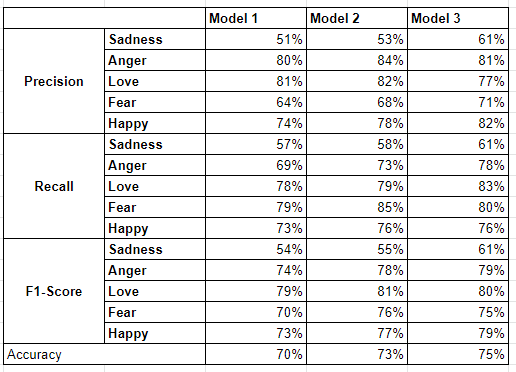
\includegraphics[width= 0.9\linewidth]{template-paper-ieee-main/gambar/3.stemming_non_freeze.png}
        \caption{Experimental results of \textit{Stemming} method and without using \textit{Freeze Parameter} using 3 \textit{Pretrained Model}}
        \label{fig: bertToken}
    \end{center}
\end{figure}

In the experiment using the \textit{Stemming} dataset and without using the \textit{Freeze Parameter}, several results were obtained from the three \textit{Pretrained Model} used. The first using the \textit{akahana/indonesia-emotion-roberta} model, the results are much different from the 2 datasets that have been tested previously with an accuracy of 70\% where this result is very far from the first two experiments using the same model with an accuracy of 90 \%. Then for the values of \textit{Precision}, \textit{Recall}, and \textit{F1-Score} are also classified as getting \textit{Range} which is quite small with a range of 51\% to 81\%. Then for the difference in \textit{Loss} itself, \textit{Training Loss} always decreases with increasing \textit{epoch} and \textit{Eval Loss} also shows the same result, but for \textit{Eval Loss} the decrease is not too drastic like \textit{Training Loss}.

The second experiment using \textit{Pretrained Model} from \textit{indolem/indobertweet-base-uncased} and the results obtained with an accuracy of 73\%. There is also a decrease from the experiment with the \textit{Non-Stemming} dataset, but it is not significant considering that it only decreases by 4\% to 5\%. Then for the range of values \textit{Metrics} \textit{Precision}, \textit{Recall}, and \textit{F1-Score}, the results are almost the same as experiments with the previous 2 dataset types with a value range of 53\% to with 85\%. For the difference in \textit{Loss} from this experiment, \textit{Training Loss} always decreases with increasing \textit{Epoch} while \textit{Eval Loss} as \textit{Epoch} increases, there is a moment where the value increases but after back down.

The third experiment using \textit{Pretrained Model} from \textit{StevenLimcorn/indonesian-roberta-base-emotion-classifier} and the results obtained with an accuracy of 75\%. There is also a significant decrease from experiments with the \textit{Non-Stemming} dataset considering that experiments with the previous 2 datasets yielded an accuracy of 88\%. Then for the range of values \textit{Metrics} \textit{Precision}, \textit{Recall}, and \textit{F1-Score} shows the results with a value range of 61\% to 83\%. For the difference in \textit{Loss} from this experiment, \textit{Training Loss} always decreases with increasing \textit{Epoch} while \textit{Eval Loss} as \textit{Epoch} increases, there is a moment where the value increases but after back down.

\subsection{Testing Dataset \textit{Stemming} and using \textit{Freeze Parameter}}

Testing with the third scheme is carried out with \textit{Dataset} which goes through the \textit{Stemming} process and without using \textit{Freeze Parameter}. In this test \textit{Dataset} goes through the \textit{Stemming} process and as a result the affixes are removed and \textit{Freeze Parameter} is used to disable some \textit{Layer} so that the model used is simpler. From the three models used, the model performance is as follows:

\begin{figure}[h]
    \begin{center}
        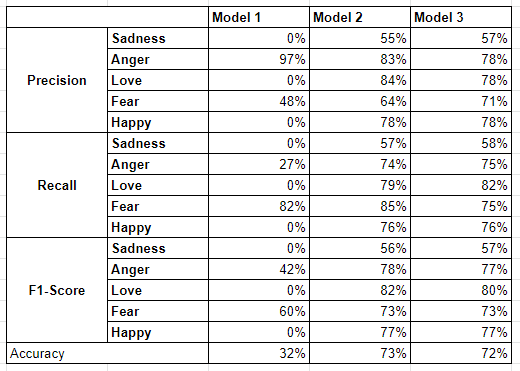
\includegraphics[width= 0.9\linewidth]{template-paper-ieee-main/gambar/4.stemming_freeze.png}
        \caption{Experiment results using \textit{Stemming} method and using \textit{Freeze Parameter} using 3 \textit{Pretrained Model}}
        \label{fig: bertToken}
    \end{center}
\end{figure}

The next experiment is using the \textit{Stemming} dataset and using the \textit{Freeze Parameter}. The first experiment using \textit{Pretraine Model} from \textit{akahana/indonesia-emotion-roberta} with poor results with the previous 3 types of datasets with an accuracy of 32\%. Then the values \textit{Precision}, \textit{Recall}, and \textit{F1-Score} show values that are smaller than the three previous dataset types with a range of 0\% to 97\%. For the difference \textit{Loss}, there is no allusion between \textit{Evaluation} and \textit{training loss} where \textit{Training Loss} is always greater than \textit{Eval Loss}.

The second experiment using \textit{Pretrained Model} from \textit{indolem/indobertweet-base-uncased} and the results obtained with an accuracy of 73\%. There is also a decrease from the experiment with the \textit{Non-Stemming} dataset, but it is not significant considering that it only decreases by 4\% to 5\%. Then for the range of values \textit{Metrics} \textit{Precision}, \textit{Recall}, and \textit{F1-Score}, the results are almost the same as experiments with the previous 2 dataset types with a value range of 55\% to with 85\%. For the difference in \textit{Loss} from this experiment, \textit{Training Loss} always decreases with increasing \textit{Epoch} while \textit{Eval Loss} always stagnates as \textit{Epoch} increases.

The third experiment using \textit{Pretrained Model} from \textit{StevenLimcorn/indonesian-roberta-base-emotion-classifier} and the results obtained with an accuracy of 72\%. There is also a significant decrease from experiments with the \textit{Non-Stemming} dataset considering that experiments with the previous 3 datasets yielded an accuracy of 88\% for \textit{Non Stemming} and and 75\% for \textit{Stemming} . Then for the range of values \textit{Metrics} \textit{Precision}, \textit{Recall}, and \textit{F1-Score} shows the results with a value range of 57\% to 82\%. For the difference in \textit{Loss} from this experiment, \textit{Training Loss} always decreases with increasing \textit{Epoch} while \textit{Eval Loss} as \textit{Epoch} increases, there is a moment where the value increases but after back down.